%% Slides for ".NET Programming" by Chunyu Wang <chunyu@hit.edu.cn> %%

\part{课程简介}

\section{联系方式}
\begin{frame}
\frametitle{联系方式}
\begin{itemize}
\setlength{\itemsep}{8pt plus 1pt}
\item 电子邮件
  \begin{itemize}
  \item chunyu@hit.edu.cn
  \end{itemize}
% \item 主页
%   \begin{itemize}
%   \item \href{http://www.emacs.cn/~chunyu}{http://www.emacs.cn/\char126chunyu}
%   \end{itemize}
\item 电话
  \begin{itemize}
  \item 13766837420 (M)
  \item 86413213 (O)
%  \item 86232865(H)
  \end{itemize}
\item 办公室
  \begin{itemize}
  \item 软件基础教研室
  \item 综合楼 415
  \end{itemize}
\end{itemize}
\end{frame}

\section{课程简介}

\begin{frame}
\frametitle{课程简介}

\CJKindent 了解 .NET 框架的功能,学习 C\# 语言,学习 .NET 框架类库, 学习
.NET 框架的开发。

\begin{itemize}
\item .NET 平台和 C\# 语言
\begin{itemize}
\item .NET 框架,公共语言运行时,$\ldots$
\item C\# 语言,类型基础,面向对象开发,$\ldots$
\end{itemize}
\item 框架类库基础
  \begin{itemize}
  \item 文件 I/O,数据流,$\ldots$
  \item 多线程,网络编程,$\ldots$
  \end{itemize}
\item 图形界面开发
\item ADO.NET
\item ASP.NET
\end{itemize}
\end{frame}

\section{课程实验}
\begin{frame}
\frametitle{课程实验}
\begin{itemize}
    \setlength{\itemsep}{14pt plus 1pt}
% \item 时间:$\cdots$
 \item 时间:3--7周, 周三、五 9~10节
% \begin{itemize}
%   \setlength{\itemsep}{6pt plus 1pt}
% \item %周六5--6节,080310\{1, 2, 3, 4\}班
% \item %周六7--8节,080310\{5, 6, 7\}, 0836111班
% \end{itemize}
\item 地点:致知楼 D01
\item 实验环境
\begin{itemize}
    \setlength{\itemsep}{6pt plus 1pt}
\item .NET Framework SDK --- 命令行工具
\item Visual Studio .NET --- 集成开发环境
\end{itemize}
\item 实验内容:
  \begin{itemize}
  \item 乐学网: \href{http://cms.hit.edu.cn/course/view.php?id=236}{http://cms.hit.edu.cn/course/view.php?id=236}
  \item 课程名: .NET程序设计
  \end{itemize}
\end{itemize}

\end{frame}

\section{参考资料}
\begin{frame}[t]
\frametitle{参考资料}

\begin{columns}
  \column{.47\textwidth}
  \begin{itemize}
  \item \small 《\textit{C\#} 和 \textit{.NET} 核心技术》\\
    ``\textit{Core C\# and .NET}''
    \begin{itemize}
    \item Stephen C. Perry 著
    \item 肖斌\ 王小振\ 等译
    \item 机械工业出版社
    \end{itemize}
    \begin{figure}
      \centering
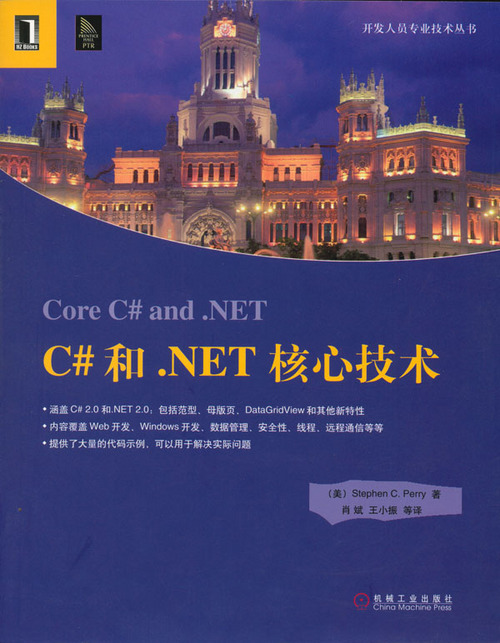
\includegraphics[width=3.5cm]{bk-corecs.jpg}
    \end{figure}
  \end{itemize}

  \column{.53\textwidth}
  \begin{itemize}
  \item 《\textit{.NET} 组件开发》(影印版)\\
 ``\textit{Programming .NET Components}''
    \begin{itemize}
    \item Juval L\"owy 著
    \item 东南大学出版社
    \end{itemize}
    \begin{figure}
      \centering
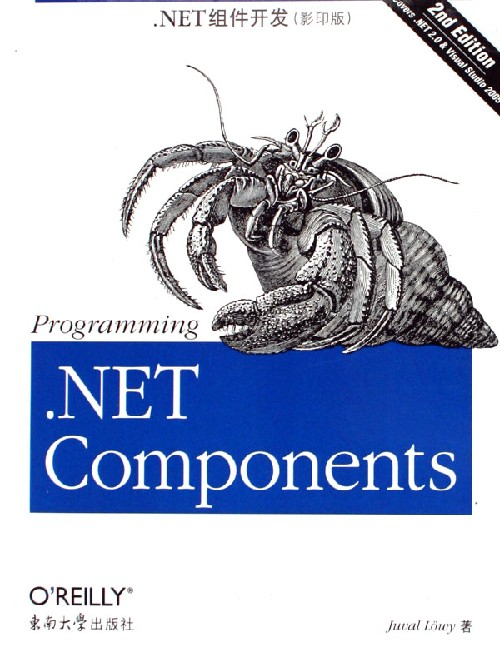
\includegraphics[width=3.5cm]{bk-dncomp.jpg}
    \end{figure}
  \end{itemize}
\end{columns}
\end{frame}

\begin{frame}[t]
\frametitle{参考资料}

\begin{itemize}
\item 《\textit{C\#} 编程语言(第2版)》(影印版)\\
  ``\textit{The C\# Programming Language}'' Second Edition
  \begin{itemize}
  \item Anders Hejlsberg, Scott Wiltamuth, Peter Golde 著
  \item 人民邮电出版社
  \end{itemize}
  \begin{figure}
    \centering
    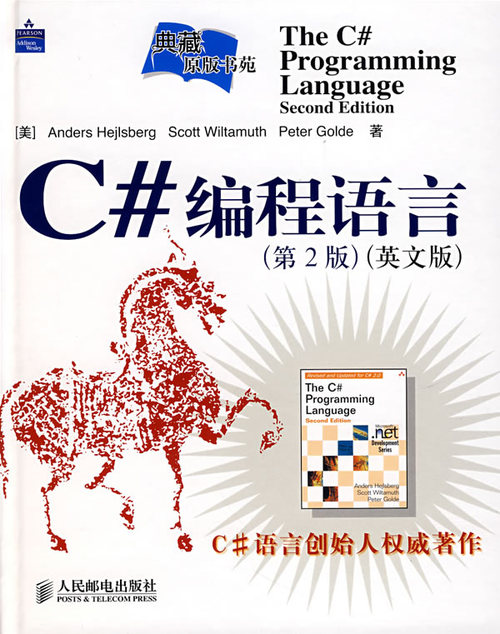
\includegraphics[width=3.5cm]{bk-thecpl.jpg}
  \end{figure}
\end{itemize}
\end{frame}

\begin{frame}
\frametitle{资源下载}
\begin{itemize}
  \setlength{\itemsep}{.4cm plus 1pt}
\item 乐学网 \href{http://cms.hit.edu.cn/course/view.php?id=236}{http://cms.hit.edu.cn/course/view.php?id=236}
  \begin{itemize}
    \setlength{\itemsep}{.2cm plus 1pt}
  \item 课件、实验指导下载
  \item 电子书
  \end{itemize}
\item ftp://run.hit.edu.cn -- \textit{202.118.224.241}
  \begin{itemize}
    \setlength{\itemsep}{.2cm plus 1pt}
  \item /software/ByCompany/Microsoft
  \item /study/Computer\_Science/programming\_language
  \end{itemize}
\item ftp://ftp.cs.hit.edu.cn
\item http://msdn.microsoft.com
\end{itemize}

\end{frame}

% Local Variables:
% mode: LaTeX
% TeX-master: "part-00.tex"
% TeX-header-end: "% End-of-Header$"
% TeX-trailer-start: "% Start-of-Trailer$"
% coding: utf-8
% End:

